\chapter{The Mechanical Origin of Mass}

\section{The Singularity Paradox}
The current synthesis of physics suffers from a fundamental incompatibility. Quantum Mechanics treats particles as dimensionless points, while General Relativity predicts that zero-volume mass must collapse into a singularity (infinite density). Standard physics resolves this only by mathematical renormalization. This suggests that the ``Point Particle'' is not a physical reality, but an approximation that breaks down at the fundamental scale.

\section{The Surface State Hypothesis}
Building on the Spacetime Gravitational Floor (SGF) architecture and Definition III (Matter), we propose that matter is not an entity distinct from space, but a Topological Defect of the vacuum structure itself.

We distinguish the support structure from the defect: 
\begin{itemize}
    \item \textbf{The Core (The Node):} The lattice node ($r_D \approx 10^{-26} \text{ m}$) acts as the rigid, phase-locked support structure. 
    \item \textbf{The Defect (The Matter):} Matter exists as a localized twist or knot on the 2D boundary layer of these cores.
\end{itemize}

\section{The Three Faces of Mass}
In Tension Field Theory (TFT), ``Mass'' is a composite mechanical property. We distinguish three functional aspects of matter: 
\begin{itemize}
    \item \textbf{Static Mass (Gravity):} The tension the defect exerts on the surrounding lattice. 
    \item \textbf{Dynamic Mass (Identity):} The Vibrational State of the lattice node. The specific Effective Displacement Volume ($V_{eff}$) defines the particle species. 
    \item \textbf{Kinematic Mass (Inertia):} The resistance to motion caused by interstitial condensate drag and lattice reconfiguration.
\end{itemize}

\section{The Mechanism of Hydrodynamic Drag}
As established in Definition III, inertial mass is generated by the viscous resistance of the Interstitial Vacuum Condensate. This formulation ($m \propto \rho_{IC} \cdot V_{eff} \cdot \sin(\Delta\phi)$) relies on a critical mechanical distinction between the two phases of the vacuum:  
\begin{itemize}
    \item \textbf{The Node ($\rho_D$):} Provides the Elastic Stiffness that sustains the internal vibration ($E = M_D c_E^2$). 
    \item \textbf{The Condensate ($\rho_{IC}$):} Provides the Viscous Resistance that creates external Inertia ($F = ma$).
\end{itemize}

\textbf{Conclusion:} A fundamental particle possesses no intrinsic mass; it possesses only an intrinsic geometric frequency ($f_{mass} = \frac{c_E}{2r_D}$, derived in Appendix \ref{app:particle_amplitude}). Mass is merely the external, macroscopic drag coefficient generated when this internal frequency forces the node's boundary to pulse against the interstitial vacuum condensate. It is strictly an interaction property.

\section{The Amplitude Hierarchy (Radius vs. Amplitude)}
Because all fundamental particles reside on lattice nodes of the exact same physical size ($r_D \approx 10^{-26} \text{ m}$) and operate at the exact same internal frequency, the hierarchy of particle masses is solely determined by their vibrational intensity. (See Appendix \ref{app:particle_amplitude} for the derivation of vibration amplitudes from vacuum condensate).

\begin{itemize}
    \item \textbf{The Top Quark ($m \approx 173 \text{ GeV}$):} Vibrates at Maximum Amplitude. The node's boundary expands and contracts with a displacement ($r_{amp}$) occupying 30.8\% of the available interstitial clearance. It acts as a ``Shout,'' displacing maximum condensate and generating massive hydrodynamic drag.
    \item \textbf{The Electron ($m \approx 0.5 \text{ MeV}$):} Vibrates at Minimum Amplitude. The node shivers with a displacement of only $10^{-33} \text{ m}$ ($r_{amp} \ll r_D$). It acts as a ``Whisper,'' displacing negligible condensate and generating minimal macroscopic drag.
\end{itemize}

\textbf{Standard Model Reinterpretation:} The Standard Model treats the electron as a dimensionless point to fit observational data and avoid infinities. TFT reinterprets this ``smallness'' not as a physical radius (the physical node remains large at $r_D$), but as a minimal vibrational amplitude ($r_{amp}$). The particle only appears point-like to our macroscopic instruments because its volumetric displacement of the vacuum condensate is infinitesimally small.

\begin{figure}[H]
    \centering
    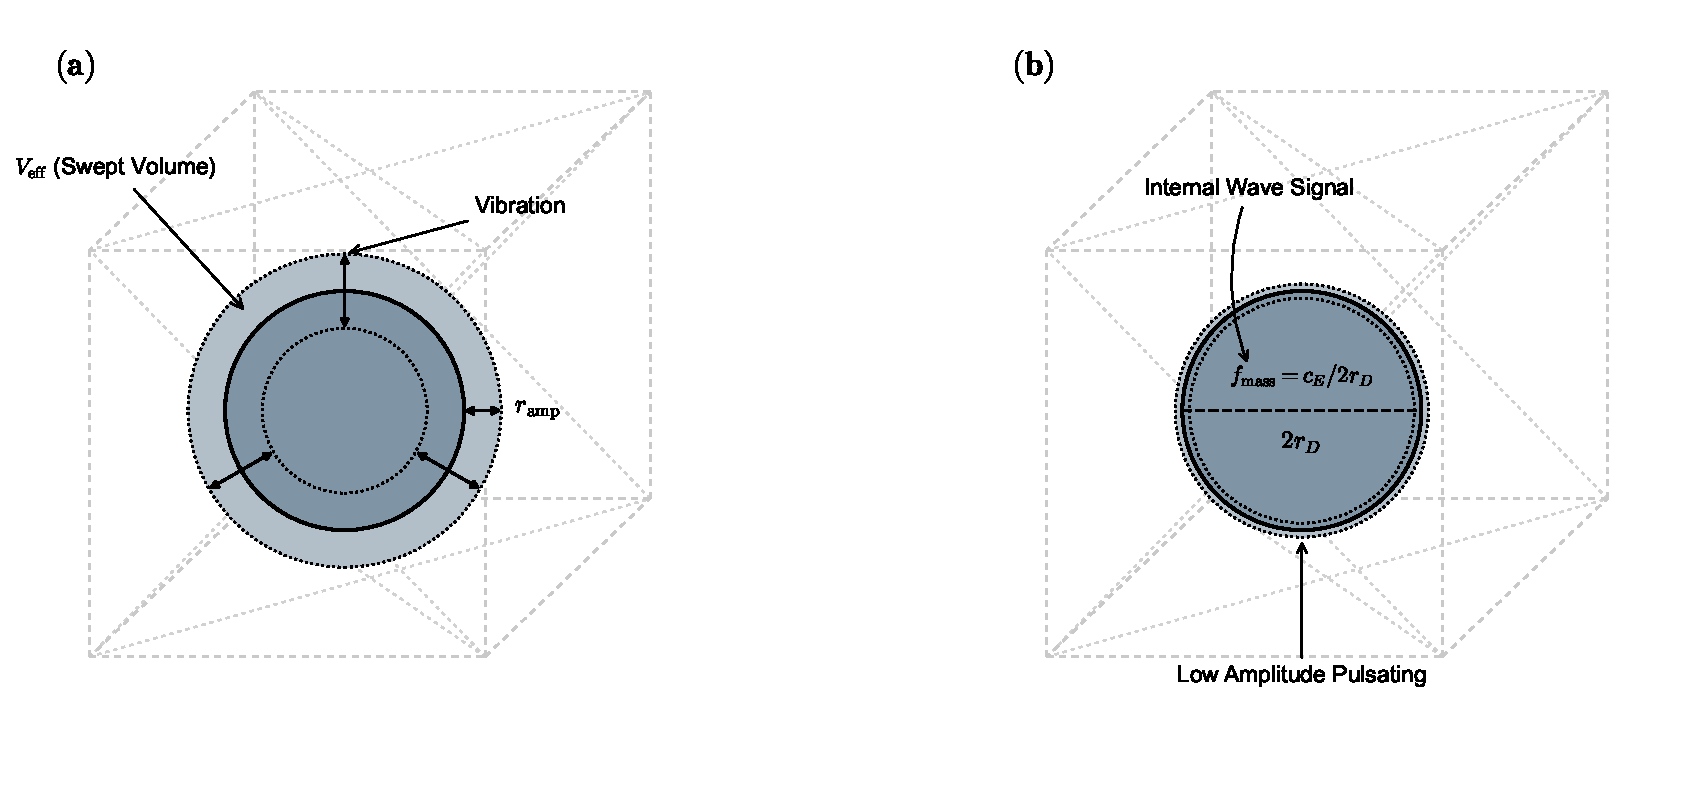
\includegraphics[width=0.9\textwidth]{Figures/Fig04_PartI_Massmechanism.pdf}
    \caption{\textbf{Deterministic Mass via Radial Displacement.} A mechanical comparison of fundamental particles (Top Quark and Electron) as topological defects within the FCC Soft Floor. Both particles share a constant structural node radius ($r_D \approx 10^{-26} \text{ m}$) and an identical internal geometric wave signal ($f_{mass} = \frac{c_E}{2r_D}$). Inertial mass emerges strictly from the coupled interaction between the active node and the passive condensate. It is the quantitative measure of the hydrodynamic drag generated by the node's external radial pulsating mode, where the effective swept volume is $V_{eff} \approx (4\pi r_D^2) \cdot r_{amp}$, yielding $m = \rho_{IC} \cdot V_{eff}$. 
    \textbf{(a) The Top Quark (Vibrational Limit Regime):} Operating as a high-amplitude ``shout,'' the top quark's vibrational amplitude ($r_{amp(t)} \approx 0.31r_D$) consumes 30.8\% of the fundamental node's internal vibrational capacity. This massive radial sweep generates extreme hydrodynamic drag, defining the absolute mass generation limit of the vacuum. 
    \textbf{(b) The Electron (High-Resolution Linear Regime):} Operating as a low-amplitude ``whisper,'' the electron's minimal vibrational scale ($r_{amp(e)} \approx 432\ell_S$) sweeps a negligible volume of the condensate. This extreme low-amplitude pulsation ($r_{amp} \ll r_D$) perfectly explains the electron's apparent dimensionless, point-like nature under current experimental resolution.}
    \label{fig:mass_mechanism}
\end{figure}

\section{Topological Stability and Conservation}
\begin{itemize}
    \item \textbf{Creation (Topological Locking):} Mass is formed when lattice vibration is confined into a self-sustaining resonance loop. This transition converts linear wave propagation into a localized standing wave ($\Delta\phi \neq 0$), trapping the energy as structural tension.
    \item \textbf{Destruction (Phase Cancellation):} Mass is annihilated when a topological knot encounters its inverse (Antimatter). The positive phase shift ($+\Delta\phi$) and negative phase shift ($-\Delta\phi$) cancel precisely, releasing the stored structural tension back into the lattice as pure vibration (Photons).
\end{itemize}

\section{The Resolution of Wave-Particle Duality}
Standard Quantum Mechanics treats wave-particle duality as an unresolved paradox, where an entity magically collapses from a smeared-out probability wave into a solid point upon measurement. Tension Field Theory eliminates this paradox by separating internal kinematics from external lattice mechanics. Duality is not a physical transformation; it is simply the distinction between what the topological defect is and what it does.

\begin{itemize}
    \item \textbf{The Wave Nature (Internal Kinematics):} Intrinsically, a fundamental particle is an oscillation of an FCC node. It is a topological phase-twist locked in a permanent standing resonance ($f_{mass} = \frac{c_E}{2r_D}$) propagating through the contiguous FCC lattice. Because the SGF nodes are permanently bonded in a Face-Centered Cubic (FCC) geometry, they cannot move independently. Instead, the twist is mechanically transferred from node to node. As it moves, this internal propagation naturally exhibits classical wave behaviors, such as phase interference and diffraction.
    \item \textbf{The Particle Nature (External Drag):} Extrinsically, this trapped wave must physically interact with its environment. As the internal phase-twist cycles, it forces the physical boundary of the node to radially pulse ($r_{amp}$), violently displacing the surrounding interstitial condensate. This localized volumetric displacement creates extreme hydrodynamic drag (inertia). When this defect strikes a detector, it does not wash over it like a wave; it transfers its inertial drag as a discrete, concentrated kinetic impact.
\end{itemize}

\textbf{Conclusion:} It never stops being a wave, and it never becomes a solid ball. The ``Wave'' is the internal kinematic propagation of the lattice node; the ``Particle'' is the discrete macroscopic impact produced when that node's vibrational amplitude ($r_{amp}$) pushes against the vacuum condensate.

\chapter{Geometric Derivation of the Cosmic Energy Budget}

\section{The Principle of Maximal Stability}
In Section 2.1 (The Zeroth Law), we established that the cosmos is formed from a contiguous tension substrate. In Section 3.4, we identified the emergent structure as a Face-Centered Cubic (FCC) lattice. We now derive the specific partitioning of energy within this geometry from first principles.

We postulate that the active vacuum, in its ground state, seeks the configuration of maximum mechanical stability. In granular mechanics, stability is achieved through Geometric Locking (Hyperstatic Rigidity). For spherical energy nodes in Euclidean 3D space, this condition necessitates the densest possible packing arrangement to minimize interstitial potential.

\section{The Kepler Conjecture and Lattice Packing}
The structural limit of the vacuum is governed by the Kepler Conjecture. This theorem establishes that no arrangement of equal-sized spheres in three-dimensional space can exceed the density of the Face-Centered Cubic (FCC) lattice (the solid nodes visually mapped in Figure \ref{fig:fcc_lattice}).

To maintain Hyperstatic Rigidity (Coordination Number = 12), the SGF must adopt this configuration. We define the geometric packing fraction ($\beta_{geo}$) of the active Spacetime Gravitational Floor (SGF) as the ratio of the volume of the solid lattice spheres ($V_{spheres}$) to the volume of the unit cell ($V_{cell}$).

For an FCC lattice with sphere radius $r$:
\begin{itemize}
    \item \textbf{Volume of spheres:} The unit cell comprises portions of spheres (8 corners at 1/8 each + 6 faces at 1/2 each) yielding a total equivalent volume of 4 spheres:
    \begin{equation}
        V_{spheres} = 4 \cdot \left(\frac{4}{3}\right)\pi r^3 = \frac{16}{3} \pi r^3
    \end{equation}
    \item \textbf{Volume of unit cell:} The edge length $a$ is related to the radius by $a = 2\sqrt{2} r$:
    \begin{equation}
        V_{cell} = a^3 = (2\sqrt{2} r)^3 = 16\sqrt{2} r^3
    \end{equation}
\end{itemize}

\section{Derivation of the Vacuum Constant}
Dividing the solid volume by the total volume yields the fundamental geometric constant of the vacuum:
\begin{equation}
    \beta_{geo} = \frac{V_{spheres}}{V_{cell}} = \frac{\frac{16}{3} \pi r^3}{16\sqrt{2} r^3} = \frac{\pi}{3\sqrt{2}} = \frac{\pi}{\sqrt{18}}
\end{equation}
Numerical value:
\begin{equation}
    \beta_{geo} \approx 0.74048
\end{equation}

\section{Identification of Dark Energy and Dark Matter}
Standard cosmology observes that Dark Energy accounts for approximately 69\% of the universe, while Dark Matter is $\approx 26\%$ and Baryonic Matter is $\approx 5\%$. TFT derives these values directly from the FCC geometry established in Section 3.4, substituting the phenomenological density parameter ($\Omega$) with the strict geometric packing fraction ($\beta$):

\begin{itemize}
    \item \textbf{Dark Energy ($\beta_\Lambda$):} Identifies as the structural lattice phase (the solid nodes). The ideal unperturbed baseline is strictly $\beta_{geo} \approx 0.74$.
    \item \textbf{Dark Matter ($\beta_{IC}$):} Identifies as the interstitial condensate capacity (the void network of the FCC Soft Floor). It is the absolute geometric remainder:
    \begin{equation}
        \beta_{IC} = 1 - \beta_{geo} \approx 0.26
    \end{equation}
    \item \textbf{The Baryonic Correction ($\beta_b$):} In the observable universe, Baryonic Matter ($\approx 5\%$) emerges as a localized vibrational defect (as defined in Definition III), converting a portion of the static lattice potential into kinetic mass. This physical excitation requires volumetric displacement, reducing the effective structural energy density of the solid nodes:
    \begin{equation}
        \beta_{\Lambda,eff} \approx \beta_{geo} - \beta_b \approx 0.74 - 0.05 = 0.69
    \end{equation}
\end{itemize}

\textbf{Conclusion:} The observed cosmic energy budget is not an arbitrary distribution of exotic fields, but the structural inevitability of the vacuum geometry. It represents the Maximum Packing Limit of space itself ($\beta_\Lambda$), partitioned against the interstitial condensate ($\beta_{IC}$), and reduced only by the localized vibrational loosening caused by Matter ($\beta_b$). Thus, the universe is not ``mostly empty''---it is mechanically full.

\chapter{The Origin of Inertia, Light, and Motion}

\section{The Tension Cell: Potential vs. Kinetic}
We identify the fundamental unit of the vacuum as the Tension Cell. As established in Section 3, its structural evolution from the latent substrate to the active lattice defines the laws of motion:
\begin{itemize}
    \item \textbf{The Latent Cell (State 0 / Hard Floor):} A perfect cube of length $\ell_S$ (Substrate Lattice Spacing). It represents the absolute geometric limit. It possesses pure potential tension but, lacking geometric expansion, possesses zero intrinsic inertial density ($\mu_S \to 0$).
    \item \textbf{The Manifest Cell (State I / Soft Floor):} A resonant sphere operating at the Duality Radius ($r_D$). Here, the potential tension is geometrically captured and converted into the mass-equivalent surface inertia ($\mu_D$) of the active Soft Floor.
\end{itemize}

\section{Inertia as the Speed Regulator}
Motion is regulated by the resistance of the medium. In TFT, inertia ($\mu_{eff}$) acts as the mechanical ``brake'' on propagation speed ($c_P$).

To quantify this resistance, we first define the theoretical gravitational energy capacity ($E_G$) of an active FCC lattice node:
\begin{equation}
    E_G \approx \mu_D \cdot c_E^2 \cdot r_D^2
\end{equation}

This relationship establishes that the baseline surface inertia ($\mu_D$) is an intrinsic structural property of the vacuum lattice. Consequently, following the standard mechanical wave relation ($c_P = \sqrt{\tau_D / \mu_{eff}}$), the absolute speed of light is inversely determined by the local effective inertial density of the medium.
\section{The Two Regimes of Propagation}
This architecture creates a universe with two distinct communication channels, defined strictly by the mechanical moduli of the vacuum phases:

\textbf{A. The Entanglement Regime (Hard Floor / Longitudinal)}
\begin{itemize}
    \item \textbf{Mechanism:} Longitudinal Stress Transmission (State Transfer).
    \item \textbf{Modulus:} The Latent Substrate is perfectly rigid and incompressible ($\tau_S \to \infty$).
    \item \textbf{Dynamics:} Operating with zero intrinsic inertial density ($\mu_S \to 0$), longitudinal stress transmits instantaneously across the lattice ($c_S \to \infty$).
    \item \textbf{Physics:} This allows for Instantaneous Stress Transfer (Entanglement) and the instantaneous equilibration of the Gravitational Tension field, without transferring transverse energy.
\end{itemize}

\textbf{B. The Relativistic Regime (The Elastic Soft Floor / Transverse)}
\begin{itemize}
    \item \textbf{Mechanism:} Transverse Shear Deformation (Energy Propagation).
    \item \textbf{Modulus:} The Active Vacuum (FCC Lattice) possesses finite shear stiffness ($\tau_D$).
    \item \textbf{Dynamics:} The ``swollen'' state of the dynamic nodes creates local structural stiffness ($\tau_D$) and node interface inertial density ($\mu_D$). The vibration of these nodes creates a shear wave whose propagation speed is strictly dictated by the surface inertia ($\mu_D$), enforcing a finite kinematic limit ($c_{shear} = c_E$).
    \item \textbf{Physics:} This is Light. It carries physical information and transverse energy, but is strictly speed-limited by the surface tension and inertial density of the active FCC lattice.
\end{itemize}

\section{The Kinematic Velocity Budget}
Because the lattice possesses a finite stiffness ($\tau_D$) and inertia ($\mu_D$), there is a strict mechanical ceiling on the total kinematic capacity a node can support. This manifests as a Fixed Velocity Budget ($c_E$) that is partitioned between Internal Resonance (Mass/Proper Time) and External Translation (Spatial Motion).

We define the microscopic kinematic identity, which follows from the orthogonal decomposition of lattice displacement into translational and resonant components:
\begin{equation}
    c_E^2 = v_{ext}^2 + v_{int}^2
\end{equation}
In this framework, acceleration is experienced as a kinematic rotation: as a particle gains spatial velocity, the force-driven phase-twist rotates the node's total velocity vector from the internal resonant axis toward the spatial axis.
\begin{itemize}
    \item $v_{ext} = c_E \cos(\Delta\phi)$ \textbf{(Spatial Velocity):} The component of lattice capacity dedicated to moving the topological knot (localized phase defect) through the contiguous medium. As $\Delta\phi \to 0$, $v_{ext} \to c_E$.
    \item $v_{int} = c_E \sin(\Delta\phi)$ \textbf{(Proper Time):} The component of lattice capacity dedicated to the internal resonant oscillation of the node. As $\Delta\phi \to 0$, $v_{int} \to 0$ (As the node undergoes Kinematic Rotation toward $c_E$, this phase-offset relative to the background lattice remains invariant, but re-oriented into the spatial dimension).
\end{itemize}

\textbf{Boundary Limit:} Because $v_{int}$ represents real mechanical oscillation against the lattice restorative force, its square cannot be negative ($v_{int}^2 \ge 0$). Therefore, $v_{ext}$ is physically capped by the lattice shear limit $c_E$. Exceeding this limit would require the node to possess a non-physical (imaginary) displacement amplitude, which is a structural impossibility in a solid-state medium.

\begin{figure}[H]
    \centering
    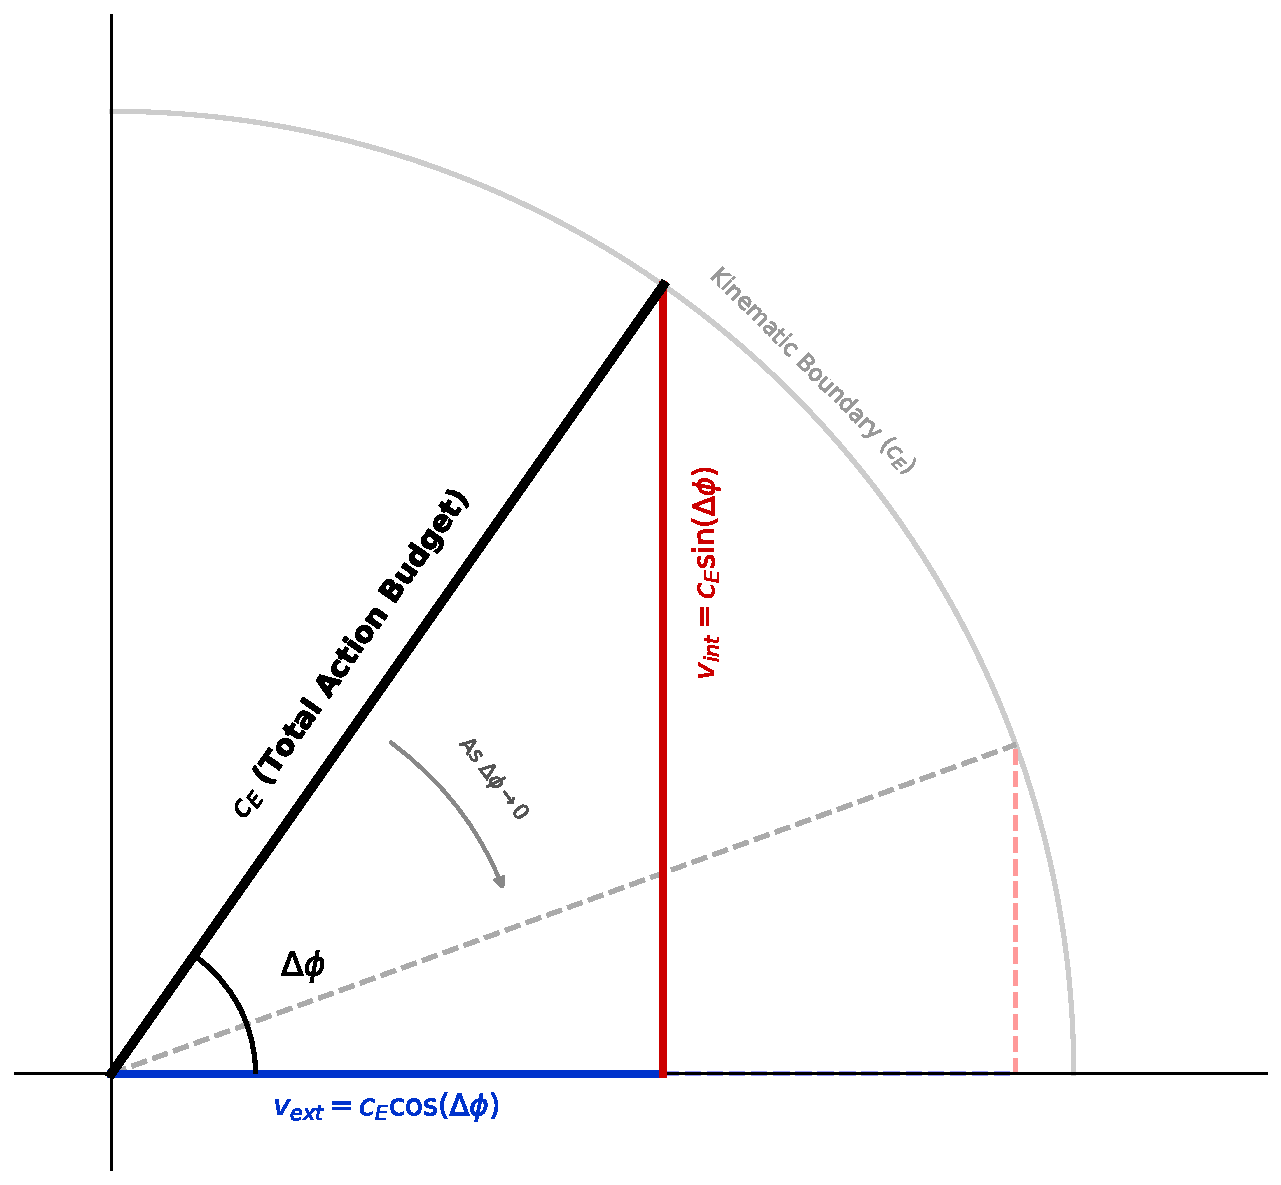
\includegraphics[width=0.8\textwidth]{Figures/Fig05_PartI_KinematicSpeedBudget.pdf}
    \caption{\textbf{The Kinematic Action Triangle.} A geometric representation of the invariant speed budget ($c_E$). Because the total action (the hypotenuse) is strictly conserved, any increase in external spatial velocity ($v_{ext}$) mechanically requires a proportional decrease in internal proper time ($v_{int}$).}
    \label{fig:kinematic_triangle}
\end{figure}

\section{The Two Mechanical States}
\textbf{The Light State (Coherence):} 
\begin{itemize}
    \item \textbf{Phase:} Adjacent nodes vibrate in near-perfect phase ($\Delta\phi \approx 0$).
    \item \textbf{Dynamics:} Near-zero phase-dissonance ensures node displacement is dominantly elastic.
    \item \textbf{Budget:} The internal cost ($v_{int}$) is zero. The entire kinematic budget is available for transmission.
    \item \textbf{Result:} The wave propagates at the maximum shear limit ($v_{ext} = c_E$). Light exhibits no internal resonant duty cycle and therefore experiences no proper-time evolution.
\end{itemize}

\textbf{The Mass State (Dissonance):} 
\begin{itemize}
    \item \textbf{Phase:} The node is a topological knot (localized phase defect) with a significant phase-angle relative to the background lattice ($\Delta\phi > 0$).
    \item \textbf{Dynamics:} This dissonance forces the node to perform work against the vacuum condensate, generating hydrodynamic resistance (Drag) that manifests macroscopically as inertia.
    \item \textbf{Budget:} This internal resonance consumes a portion of the $c_E$ budget.
    \item \textbf{Result:} The remaining capacity for spatial motion is reduced ($v_{ext} < c_E$). The particle moves slower than light because it is structurally locked into local oscillation.
\end{itemize}

\subsection*{Conclusion: The Mechanical Emergence of the Lorentz Factor}
Time dilation is a mechanical capacity partition. As $v_{ext}$ consumes the displacement bandwidth, the frequency of internal oscillation ($v_{int}$) must drop. The structural bonds are stretched toward their elastic limit, leaving less capacity for internal restorative relaxation.

By rearranging the kinematic identity, we obtain $v_{int} = \sqrt{c_E^2 - v_{ext}^2}$. The Lorentz factor ($\gamma$) naturally emerges as the ratio between the total lattice velocity budget and the remaining internal resonant capacity:
\begin{equation}
    \gamma = \frac{c_E}{v_{int}} = \frac{1}{\sqrt{1 - \frac{v_{ext}^2}{c_E^2}}}
\end{equation}

\section{Force Transfer Efficiency (Impedance Matching)}
Dynamic force is a Phase Twist ($-\nabla\phi$) transmitted across the contiguous lattice by transverse waves at speed $c_E$. The ability of this field to do work on a particle depends on the Impedance Match between the wave-front and the 3D topological defect.

The effective force delivered to a massive particle is governed by the volumetric overlap between the propagating phase-twist and the internal resonance of the defect. As the particle's internal resonant bandwidth ($v_{int}$) shrinks due to spatial motion, its structural receptivity to the lattice force-wave diminishes. The coupling efficiency follows the ratio of the available internal resonance to the total lattice budget:
\begin{equation}
    F_{effective} = F_{source} \cdot \left(\frac{v_{int}}{c_E}\right) = \frac{F_{source}}{\gamma}
\end{equation}
\begin{itemize}
    \item \textbf{At Rest ($v_{ext}=0, \gamma=1$):} Coupling is perfect ($F_{effective} = F_{source}$). This is the Newtonian Limit.
    \item \textbf{Approaching Shear Limit ($v_{ext} \to c_E, \gamma \to \infty$):} Coupling efficiency collapses to zero as the internal resonance ($v_{int}$) vanishes. This is the Saturation Limit.
\end{itemize}

\textbf{Conclusion: The Saturated Vacuum}\\
The ``relativistic'' increase in energy required for acceleration is a Mechanical Impedance Mismatch. As $v_{ext} \to c_E$, the force-transfer mechanism becomes asymptotically inefficient because the particle has no remaining resonant capacity to absorb the phase-twist. 

Crucially, the electron's mass ($m_0$) remains an invariant structural defect. The universe does not require mass to become infinite to enforce a speed limit; it simply requires the impedance of the medium to reach a saturation point. The relativistic limit is not a property of the particle, but the mechanical saturation of force-coupling in a finite-speed medium.

\begin{figure}[H]
    \centering
    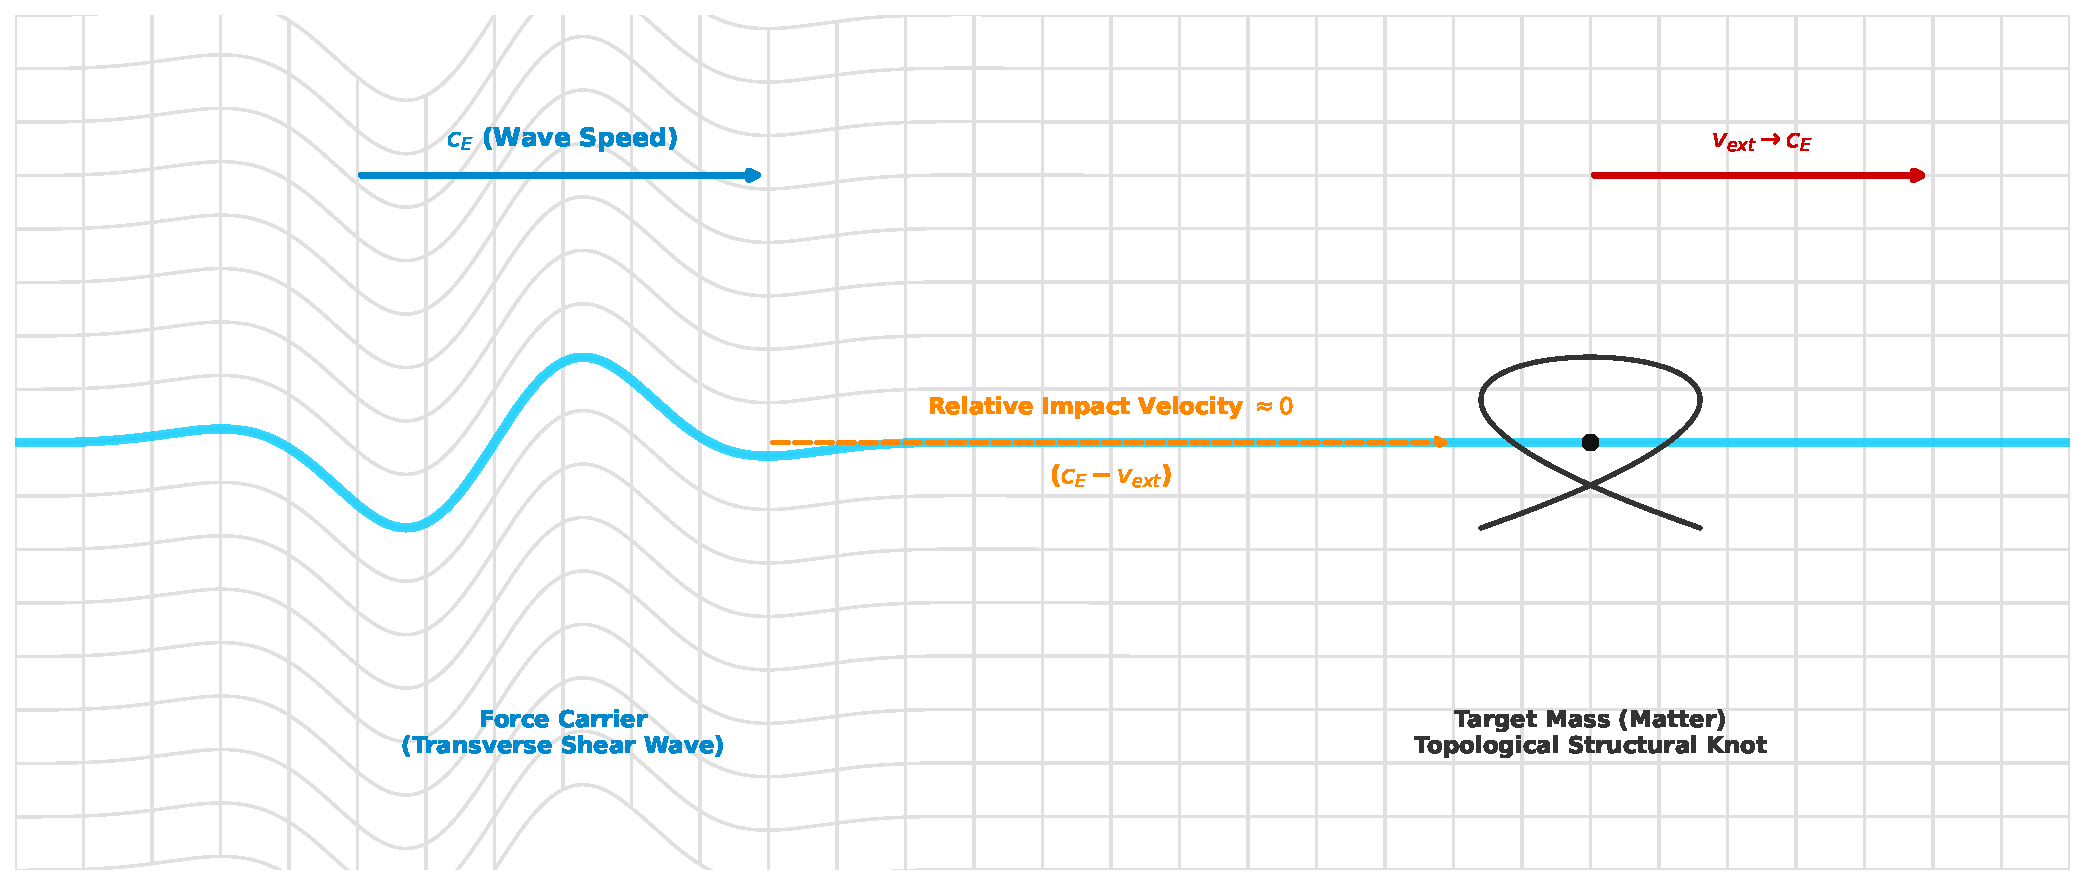
\includegraphics[width=0.8\textwidth]{Figures/Fig06_PartI_ForceCoupling.pdf}
    \caption{\textbf{Force Transfer Efficiency (The Kinematic Coupling Limit).} A visual representation of the mechanical failure of kinematic force transfer. Because the force carrier (the transverse shear wave) propagates at a fixed absolute limit ($c_E$), its ability to transfer momentum diminishes as the target's spatial velocity ($v_{ext}$) increases. As the target approaches $c_E$, the carrier can no longer catch it, causing the effective push of the vacuum ($F_{effective}$) to asymptotically drop to zero.}
    \label{fig:force_coupling}
\end{figure}

\chapter{Impedance Mismatch and the Dark Sector}

\section{The Impedance Mismatch}
The mechanical model of the SGF naturally explains the invisibility of the dark sector by distinguishing between the Solid and Fluid phases of the vacuum:

\begin{itemize}
    \item \textbf{Light (Solid Phase):} Propagates exclusively through the FCC solid surface. Solids possess \textit{Shear Stiffness} ($\tau_D > 0$), which is the requisite mechanical property for supporting transverse electromagnetic waves (photons).
    \item \textbf{Dark Matter (Fluid Phase):} Resides in the Vacuum Condensate (Liquid Voids). Liquids possess a \textit{Bulk Modulus} (allowing them to conduct longitudinal sound/gravity) but effectively exhibit zero \textit{Shear Stiffness} ($\tau_D \approx 0$).
\end{itemize}

\textbf{The Boundary Barrier:} Because the vacuum condensate cannot support shear stress, transverse light waves cannot penetrate the interstitial voids. The photons are mechanically forced to bypass or reflect off these regions entirely.

\section{Conclusion: The Mechanical Origin of Transparency}
Dark matter is ``invisible'' not because it is composed of exotic phantom particles, but because there exists an \textbf{Infinite Impedance Mismatch} for shear waves between the solid lattice (the light carrier) and the liquid voids (the mass reservoir). 

Light, being a transverse shear wave, is structurally excluded from the fluid condensate. Conversely, Gravity (represented as Tension/Pressure) is a longitudinal state of the medium that permeates both phases simultaneously. This explains why Dark Matter interacts via gravity but remains completely decoupled from the electromagnetic spectrum.